\chapter{Mathematical Background}\label{app:mathematicalbackground}

\firstwords{To say that} computer science and mathematics are closely related would be an understatement. Indeed, some of the pioneering work in computer science was done by career mathematicians in a time before ``computer scientists" even existed. The bond between these two subjects is perhaps strongest when it comes to the theory of computing: flip to any page in this book and you'll find some kind of mathematical terminology or notation.

Comfort with mathematics is necessary for success in computer science. In this appendix, we will review some of the important notions one should know in order to learn and understand the theory of computing.

\section{Sets and Sequences}

\firstwords{The concepts} underpinning almost everything we cover in this book are some of the most elementary in all of mathematics: sets and sequences.

\subsection*{Sets, Operations, and Properties}

Let us begin with a very simple definition: that of a \emph{set}.

\begin{definition}[Set]
A set is a collection of elements.
\end{definition}

If an element $a$ belongs to a set $S$, then we write $a \in S$. Otherwise, we write $a \not\in S$. Elements of a set are unique; for example, two indistinguishable copies of an element $a$ cannot belong to the same set $S$. If we require that some set contain more than one indistinguishable copy of some element, then we say that set is a \emph{multiset}.

We may describe sets either by listing their elements explicitly, or by describing some property or properties possessed by each element in the set. Of course, if the set is infinite, we typically prefer to use the latter method.

\begin{example}
Let's come up with some basic examples of sets:
\begin{itemize}
	\item The set of all Canadian host cities of the Olympics is
	\begin{equation*}
	C_{\text{Olympics}} = \{\text{Montr\'{e}al}, \, \text{Calgary}, \, \text{Vancouver}\}.
	\end{equation*}
	
	\item The set of all years in the 20th century in which the summer Olympics were held is
	\begin{equation*}
	\begin{split}
	O_{\text{1900s}} = \{&1904, 1908, 1912, 1920, 1924, 1928, 1932, \\
		&1936, 1948, 1952, 1956, 1960, 1964, 1968, \\
		&1972, 1976, 1980, 1984, 1988, 1992, 1996\}.
	\end{split}
	\end{equation*}
	
	\item The set of all prime numbers less than 20 is
	\begin{equation*}
	P_{<20} = \{2, 3, 5, 7, 11, 13, 17, 19\}.
	\end{equation*}
	
	\item The set of all positive odd integers is
	\begin{equation*}
	S_{\text{odd}} = \{n \mid n = 2k+1, k \geq 0\}.
	\end{equation*}
\end{itemize}
\end{example}

There are some sets that we use frequently enough to warrant their own notation. The set of \emph{natural numbers} is $\mathbb{N} = \{0, 1, 2, \dots\}$, and the set of \emph{integers} is $\mathbb{Z} = \{\dots, -2, -1, 0, 1, 2, \dots\}$. Occasionally, we also refer to the set of \emph{real numbers}, denoted $\mathbb{R}$, although their definition is better left for a book on real analysis. Computer scientists in particular are often interested in the set of \emph{binary digits} or \emph{bits}, sometimes denoted $\mathbb{B} = \{\texttt{0}, \texttt{1}\}$. These common sets and their relationships are depicted in Figure~\ref{fig:commonsets}.

\begin{figure}[t]
\centering
\begin{tikzpicture}
\draw[draw=\secondcolour, fill=\secondcolour, thick, rounded corners] (-2,-1) rectangle (5,3);
\draw[draw=\thirdcolour, fill=\thirdcolour, thick, rounded corners] (-1.5,-0.5) rectangle (3.5,2.5);
\draw[draw=\fourthcolour, fill=\fourthcolour, thick, rounded corners] (-1,0) rectangle (2,2);
\draw[draw=\fifthcolour, fill=\fifthcolour, thick, rounded corners] (-0.5,0.5) rectangle (0.5,1.5);

\node[color=\maincolour] at (4.25,2.25) {\huge{\color{white}$\mathbb{R}$}};
\node[color=\maincolour] at (2.75,1.75) {\huge{\color{\maincolour}$\mathbb{Z}$}};
\node[color=\maincolour] at (1.25,1.25) {\huge{\color{\maincolour}$\mathbb{N}$}};
\node[color=\maincolour] at (0.025,1) {\huge{\color{\maincolour}$\mathbb{B}$}};
\end{tikzpicture}
\caption{Some common sets and their relationships}
\label{fig:commonsets}
\end{figure}

The \emph{cardinality} or \emph{size} of a set $S$, denoted $|S|$, is equal to the number of elements in $S$. If $|S| = n$ for some finite $n \geq 0$, then we say that $S$ is a \emph{finite set}. Otherwise, we say that $S$ is an \emph{infinite set}. We say that an infinite set $S$ is \emph{countably infinite} if we can associate each element of $S$ to exactly one natural number in $\mathbb{N}$, and each natural number is associated with exactly one element of $S$; if no such association is possible, then we say that $S$ is \emph{uncountably infinite}.

The unique set with cardinality zero is called the \emph{empty set}, and we denote it by $\emptyset$. At the other extreme, the set of all elements under consideration is the \emph{universal set} or just the \emph{universe}, and is occasionally written $\mathcal{U}$.

There are a number of elementary and useful operations we can apply to sets. The \emph{union} of two sets $S$ and $T$, denoted $S \cup T$, is the set containing all elements that are in $S$ or in $T$ (or in both). The \emph{intersection} of $S$ and $T$, denoted $S \cap T$, is the set containing all elements that are in both $S$ and $T$. The \emph{complement} of a set $S$, denoted $\overline{S}$, is the set containing all elements from our universe that are not in $S$. Lastly, the \emph{difference} of $S$ and $T$, denoted $S \setminus T$, is the set of all elements of $S$ that are not also in $T$.

\begin{example}
Suppose $\mathcal{U} = \mathbb{N}$. The set of all positive even integers is
\begin{equation*}
S_{\text{even}} = \overline{S_{\text{odd}}} = \mathbb{N} \setminus S_{\text{odd}}.
\end{equation*}

\noindent
We can see that $S_{\text{odd}} \cup S_{\text{even}} = \mathcal{U}$, while $S_{\text{odd}} \cap S_{\text{even}} = \emptyset$.
\end{example}

From our example, we see that we can define our complement operation in terms of our difference operation by taking $\overline{S} = \mathcal{U} \setminus S$. As a consequence, we have that both $\overline{\mathcal{U}} = \emptyset$ and $\overline{\emptyset} = \mathcal{U}$.

Given two sets $S$ and $T$, if every element of $S$ is also an element of $T$, we say that $S$ is a \emph{subset} of $T$ and we write $S \subseteq T$. If, additionally, $T$ contains at least one element that $S$ does not contain, then we say that $S$ is a \emph{proper subset} of $T$ and we write $S \subset T$. If no element of $S$ is an element of $T$ and vice versa, then we say that $S$ and $T$ are \emph{disjoint}.

\begin{example}
Each of the following relationships between sets holds:
\begin{itemize}
	\item The set $S_{\text{odd}}$ is a proper subset of both $\mathbb{N}$ and $\mathbb{Z}$, while the sets $S_{\text{odd}}$ and $S_{\text{even}}$ are disjoint.

	\item It is possible to have chains of subsets, such as $\mathbb{B} \subset \mathbb{N} \subset \mathbb{Z} \subset \mathbb{R}$.

	\item For all sets $S$, $\emptyset \subseteq S \subseteq \mathcal{U}$.
\end{itemize}
\end{example}

\begin{remark}
The notation for indicating subset and proper subset relationships is, annoyingly, inconsistent across the literature. Here, we denote a subset relationship by the symbol $\subseteq$, analogous to how the ``less than or equal to" symbol $\leq$ indicates that the object on the right-hand side may be the same as the object on the left-hand side. Likewise, we denote a proper subset relationship by the symbol $\subset$, analogous to how the ``less than" symbol $<$ indicates that the object on the right-hand side is strictly larger than the object on the left-hand side.
\end{remark}

We can go one step further by defining \emph{set equality} in terms of subsets: we say that two sets $S$ and $T$ are \emph{equal} if both $S \subseteq T$ and $T \subseteq S$.

Lastly, the \emph{power set} of a set $S$, denoted $\mathcal{P}(S)$, is the set of all subsets of $S$. For all sets $S$, it is the case that $|S| < |\mathcal{P}(S)|$; specifically, if $S$ is a finite set, then $|\mathcal{P}(S)| = 2^{|S|}$. The power set of an infinite set always has infinite cardinality, but the power set of a countably infinite set has an uncountably infinite cardinality.

\begin{example}
Let $S = \{1, 2, 3\}$. Then
\begin{equation*}
\mathcal{P}(S) = \{\{\emptyset\}, \{1\}, \{2\}, \{3\}, \{1,2\}, \{1,3\}, \{2,3\}, \{1,2,3\}\},
\end{equation*}
and $|\mathcal{P}(S)| = 2^{3} = 8$.
\end{example}

Note that, for every set $S$, the power set $\mathcal{P}(S)$ always contains the elements $\{\emptyset\}$ and $S$ itself. It is also worth noting that $\emptyset$ and $\{\emptyset\}$ are \emph{not} the same: $\emptyset$ is the unique set with zero elements, while $\{\emptyset\}$ is a set with cardinality $1$ containing the element $\emptyset$.

\subsection*{Sequences and Operations}

In a set, ordering does not matter: as long as two sets contain the same elements, they are equal. For example, the sets $\{1, 2, 4, 8\}$ and $\{2, 8, 4, 1\}$ are equal, despite their elements not appearing in the same order. If we need to maintain or preserve some ordering in a collection of elements, we must instead use a \emph{sequence}.

\begin{definition}[Sequence]
A sequence is an ordered set of elements.
\end{definition}

We distinguish notationally between sets and sequences in the following way: sets are surrounded by $\{$braces$\}$, while sequences are surrounded by $($parentheses$)$. We further distinguish sets from sequences by appending to the sequence's label a subscripted $n$; thus, while we may denote a set by something like $S$, we will denote a sequence by something like $A_{n}$. Given a sequence $A_{n} = (a_{0}, a_{1}, a_{2}, \dots)$, we say that the element $a_{i}$ is the $i$th \emph{term} of the sequence.

We occasionally refer to a sequence having a finite length as a \emph{tuple}, or as a \emph{$k$-tuple} if we know the sequence contains $k$ terms. A sequence having a length of two is called an \emph{ordered pair}.

Unlike sets, a sequence may contain non-unique or repeated terms.

\begin{example}
Let's come up with some basic examples of sequences:
\begin{itemize}
	\item The sequence $L_{n}$ of the digits in the decimal representation of the speed of light $c$, in metres per second, is
	\begin{equation*}
	L_{n} = (2, 9, 9, 7, 9, 2, 4, 5, 8).
	\end{equation*}
	
	\item The Fibonacci sequence $F_{n}$ is defined as follows: fix $F_{0} = F_{1} = 1$. Then, for each $n \geq 2$, $F_{n} = F_{n-1} + F_{n-2}$. The first few terms of the Fibonacci sequence are
	\begin{equation*}
	F_{n} = (1, 1, 2, 3, 5, 8, 13, 21, 34, \dots).
	\end{equation*}
	
	\item The Thue--Morse sequence $T_{n}$ is defined as follows: for all $n \geq 0$, $T_{n} = 0$ if the number of ones in the binary representation of $n$ is even, and $T_{n} = 1$ if the number of ones is odd. The first few terms of the Thue--Morse sequence are
	\begin{equation*}
	T_{n} = (0, 1, 1, 0, 1, 0, 0, 1, 1, 0, 0, 1, 0, 1, 1, 0, \dots).
	\end{equation*}
\end{itemize}
\end{example}

\begin{remark}
The study of integer sequences is of keen interest to some mathematicians and computer scientists. The On-line Encyclopedia of Integer Sequences, accessible at \url{https://oeis.org}, contains over 375\,000 examples of sequences, many of which include relationships to other sequences, code snippets to generate terms of the sequence, and citations to the literature.
\end{remark}

Using the notion of sequences, we can define another set operation: the \emph{Cartesian product}. Given two sets $S$ and $T$, their Cartesian product, denoted $S \times T$, is the set of all ordered pairs where the first element of the pair comes from $S$ and the second element comes from $T$. Formally speaking, $S \times T = \{(a,b) \mid a \in S \text{ and } b \in T\}$.

\begin{example}
Let $S = \{1, 2, 3\}$ and $T = \{2, 4, 6\}$. Then
\begin{equation*}
S \times T = \{(1,2), (1,4), (1,6), (2,2), (2,4), (2,6), (3,2), (3,4), (3,6)\}.
\end{equation*}
\end{example}

We can, of course, take the Cartesian product of a set $S$ with itself: we denote this by $S \times S = S^{2}$. We can further take $S^{2} \times S = S \times S^{2} = S^{3}$, and so on. In general, taking the Cartesian product of a set $S$ with itself $k$ times is denoted $S^{k}$.

\begin{example}
Taking $\mathbb{Z} \times \mathbb{Z} = \mathbb{Z}^{2}$ yields the set of all ordered pairs of integers, which gives us the Cartesian coordinate system (otherwise known as the ``$xy$-plane").
\end{example}

\section{Relations and Functions}

\firstwords{By taking the idea} of the Cartesian product further, we can define relations and functions, which associate elements of one set $S$ to elements of another set $T$. The set $S$ is called the \emph{domain}, while the set $T$ is called the \emph{codomain}. Not all elements of $T$ need be associated to some element of $S$; elements that are associated constitute the \emph{range} of the relation or function.

\subsection*{Relations}

A \emph{relation} consists of ordered pairs from the Cartesian product $S \times T$. If $a \in S$ and $b \in T$, then the ordered pair $(a,b)$ relates $a$ and $b$.

\begin{definition}[Relation]
A relation $R$ from a set $S$ to a set $T$ is a subset of $S \times T$.
\end{definition}

\begin{example}\label{ex:relationexamples}
There are many classic examples of relations:
\begin{itemize}
\item The equality relation is taken to be
\begin{equation*}
R_{=} = \{(a,b) \in \mathbb{R} \times \mathbb{R} \mid a = b\}.
\end{equation*}
\item The less-than relation is taken to be
\begin{equation*}
R_{<} = \{(a,b) \in \mathbb{R} \times \mathbb{R} \mid a < b\}.
\end{equation*}
\item The divides relation is taken to be
\begin{equation*}
R_{\text{div}} = \{(a,b) \in \mathbb{Z} \times \mathbb{Z} \mid b = ac \text{ for some } c \in \mathbb{Z}\}.
\end{equation*}
\item The rock-paper-scissors relation is taken to be
\begin{equation*}
R_{\text{rps}} = \{(a,b) \in \{\text{r}, \text{p}, \text{s}\} \times \{\text{r}, \text{p}, \text{s}\} \mid a \text{ beats or ties } b\}.
\end{equation*}
\end{itemize}
\end{example}

We have assumed in our examples that relations are between two sets; that is, they are \emph{binary} relations. We can generalize from binary relations to $k$-ary relations in the usual way.

\begin{example}
Let's come up with some examples of relations having an arity greater than two:
\begin{itemize}
\item Let $P$ be the set of professors, let $C$ be the set of courses, and let $T = \{\text{fall}, \text{winter}\}$ be the set of academic terms. Define a relation $R_{\text{sched}} \subseteq P \times C \times T$ where a tuple $(p,c,t) \in R_{\text{sched}}$ indicates that professor $p$ is teaching course $c$ in term $t$.

	(Finding the complete set of tuples in $R_{\text{sched}}$ is left as an exercise for the Registrar's Office.)
	
\item Let $N$ be the set of names of people, let $O$ be the set of origin airports, let $D$ be the set of destination airports, and let $F$ be the set of flight numbers. Define a relation $R_{\text{flight}} \subseteq N \times O \times D \times F$ where a tuple $(n, o, d, f) \in R_{\text{flight}}$ indicates that person $n$ flew from airport $o$ to airport $d$ via the flight $f$.
\end{itemize}
\end{example}

We can define a number of properties of a relation $R$ depending on which ordered pairs belong to the relation. Let $a$, $b$, and $c$ each be elements. Then
\begin{colouredbox}
\begin{itemize}
\item $R$ is \emph{reflexive} if, for all $a$, $(a, a) \in R$;
\item $R$ is \emph{symmetric} if $(a, b) \in R$ implies $(b, a) \in R$;
\item $R$ is \emph{antisymmetric} if $(a, b) \in R$ and $(b, a) \in R$ implies $a = b$; and
\item $R$ is \emph{transitive} if $(a, b) \in R$ and $(b, c) \in R$ implies $(a, c) \in R$.
\end{itemize}
\end{colouredbox}

\noindent
Despite their names, the properties of symmetry and antisymmetry are not mutually exclusive. A relation may be both symmetric and antisymmetric.

\begin{example}
Returning to our classic relations from Example~\ref{ex:relationexamples}, we see that:
\begin{itemize}
\item the equality relation $R_{=}$ is 
	\begin{itemize}
	\item reflexive since $a = a$ for all $a$, 
	\item symmetric since $a = b$ implies $b = a$ for all $a$ and $b$, 
	\item antisymmetric since both $a = b$ and $b = a$ implies that $a$ and $b$ are the same element, and 
	\item transitive since $a = b$ and $b = c$ implies that $a = c$ for all $a$, $b$, and $c$;
	\end{itemize}
\item the less-than relation $R_{<}$ is 
	\begin{itemize}
	\item not reflexive since $a \not< a$ for any $a$, 
	\item not symmetric since $a < b$ does not imply that $b < a$ for any $a$ or $b$, 
	\item not antisymmetric since it is impossible to have both $a < b$ and $b < a$, and 
	\item transitive since $a < b$ and $b < c$ implies that $a < c$ for all $a$, $b$, and $c$;
	\end{itemize}
\item the divides relation $R_{\text{div}}$ is 
	\begin{itemize}
	\item reflexive since $a$ divides $a$ for all $a$, 
	\item not symmetric since $a$ dividing $b$ does not imply that $b$ divides $a$ for all $a$ and $b$, 
	\item antisymmetric since both $a$ dividing $b$ and $b$ dividing $a$ implies that $a$ and $b$ are the same element, and 
	\item transitive since $a$ dividing $b$ and $b$ dividing $c$ implies that $c = kb = k(\ell a) = (k\ell)a$ for some $k, \ell \in \mathbb{Z}$; and
	\end{itemize}
\item the rock-paper-scissors relation $R_{\text{rps}}$ is
	\begin{itemize}
	\item reflexive since $a$ ties $a$ for all $a$,
	\item not symmetric since $a$ beating or tying $b$ does not imply that $b$ beats or ties $a$ for all $a$ and $b$,
	\item antisymmetric since both $a$ tying $b$ and $b$ tying $a$ implies that $a$ and $b$ are the same element, and
	\item not transitive since (for example) rock beating scissors and scissors beating paper does not imply that rock beats paper.
	\end{itemize}
\end{itemize}
\end{example}

\subsection*{Functions}

A \emph{function} from a set $S$ to a set $T$ is a special kind of relation where each element of $S$ is mapped to exactly one element of $T$. All functions are relations, but not all relations are functions.

\begin{definition}[Function]
A function $f$ from a set $S$ to a set $T$ is a subset of $S \times T$ such that, for each $a \in S$, there exists exactly one $b \in T$ such that $(a,b) \in f$.
\end{definition}

If $f$ is a function from a set $S$ to a set $T$, then we often denote this by the shorthand notation $f \from S \to T$, where the colon is taken to mean ``from" and the arrow is taken to mean ``to". If $(a,b) \in f$, then we write $f(a) = b$.

\begin{example}\label{ex:functionexamples}
There are many classic examples of functions $f \from \mathbb{N} \to \mathbb{N}$:
\begin{itemize}
\item The constant function, $f(x) = c$ for some $c \in \mathbb{N}$, where \\ $f(0) = c$, $f(1) = c$, $f(2) = c$, $f(3) = c$, $f(4) = c$, $f(5) = c$, \dots.
\item The integer division function, $f(x) = \lfloor x/2 \rfloor$, where \\ $f(0) = 0$, $f(1) = 0$, $f(2) = 1$, $f(3) = 1$, $f(4) = 2$, $f(5) = 2$, \dots.
\item The linear function, $f(x) = x$, where \\ $f(0) = 0$, $f(1) = 1$, $f(2) = 2$, $f(3) = 3$, $f(4) = 4$, $f(5) = 5$, \dots.
\item The quadratic function, $f(x) = x^{2}$, where \\ $f(0) = 0$, $f(1) = 1$, $f(2) = 4$, $f(3) = 9$, $f(4) = 16$, $f(5) = 25$, \dots.
\item The exponential function, $f(x) = 2^{x}$, where \\ $f(0) = 1$, $f(1) = 2$, $f(2) = 4$, $f(3) = 8$, $f(4) = 16$, $f(5) = 32$, \dots.
\end{itemize}
\end{example}

Functions are sometimes expressed visually by way of a \emph{bubble diagram}, wherein the two sets $S$ and $T$ are represented by two large ellipses and elements within each set are represented by smaller circles. If $f(a) = b$ for some elements $a \in S$ and $b \in T$, then this is depicted by an arrow in the bubble diagram. An example of a bubble diagram is shown in Figure~\ref{fig:bubblediagram}.

\begin{figure}
\centering
\begin{tikzpicture}[node distance=2cm, >=latex, every state/.style={fill=white}]
\draw[draw=\fourthcolour, fill=\fourthcolour] (-2, 0) ellipse (1cm and 2cm);
\draw[draw=\fourthcolour, fill=\fourthcolour] (2, 0) ellipse (1cm and 2cm);

\node[ellipse, draw=none] (aS) at (-2, 1.35) {\color{\maincolour}\large$S$};
\node[ellipse, draw=\thirdcolour, fill=\thirdcolour] (a1) at (-2, 0.6) {};
\node[ellipse, draw=none] (a1l) at (-2.4, 0.6) {\color{\maincolour}\small$a_{1}$};
\node[ellipse, draw=\thirdcolour, fill=\thirdcolour] (a2) at (-2, -0.1) {};
\node[ellipse, draw=none] (a2l) at (-2.4, -0.1) {\color{\maincolour}\small$a_{2}$};
\node[ellipse, draw=\thirdcolour, fill=\thirdcolour] (a3) at (-2, -0.8) {};
\node[ellipse, draw=none] (a3l) at (-2.4, -0.8) {\color{\maincolour}\small$a_{3}$};
\node[ellipse, draw=none] (ad) at (-2, -1.4) {\color{\maincolour}$\vdots$};

\node[ellipse, draw=none] (aS) at (2, 1.35) {\color{\maincolour}\large$T$};
\node[ellipse, draw=\thirdcolour, fill=\thirdcolour] (b1) at (2, 0.6) {};
\node[ellipse, draw=none] (b1l) at (2.45, 0.6) {\color{\maincolour}\small$b_{1}$};
\node[ellipse, draw=\thirdcolour, fill=\thirdcolour] (b2) at (2, -0.1) {};
\node[ellipse, draw=none] (b2l) at (2.45, -0.1) {\color{\maincolour}\small$b_{2}$};
\node[ellipse, draw=\thirdcolour, fill=\thirdcolour] (b3) at (2, -0.8) {};
\node[ellipse, draw=none] (b3l) at (2.45, -0.8) {\color{\maincolour}\small$b_{3}$};
\node[ellipse, draw=none] (bd) at (2, -1.4) {\color{\maincolour}$\vdots$};

\draw[-Latex, thick, shorten >=0.25cm, shorten <=0.25cm, color=\maincolour] (a1.east) -- (b2.west);
\draw[-Latex, thick, shorten >=0.25cm, shorten <=0.25cm, color=\maincolour] (a2.east) -- (b3.west);
\draw[-Latex, thick, shorten >=0.25cm, shorten <=0.25cm, color=\maincolour] (a3.east) -- (b1.west);
\end{tikzpicture}
\caption{An example of a bubble diagram}
\label{fig:bubblediagram}
\end{figure}

Similar to relations, we can define a number of properties of a function $f$ from a set $S$ to a set $T$.
\begin{colouredbox}
\begin{itemize}
\item $f$ is \emph{injective} (or \emph{one-to-one}) if, for all $a_{1}, a_{2} \in S$ where $a_{1} \neq a_{2}$, $f(a_{1}) \neq f(a_{2})$;
\item $f$ is \emph{surjective} (or \emph{onto}) if, for all $b \in T$, there exists $a \in S$ such that $f(a) = b$; and
\item $f$ is \emph{bijective} if it is both injective and surjective.
\end{itemize}
\end{colouredbox}
\noindent
Examples of each type of function are illustrated in Figure~\ref{fig:functiontypes}.

\begin{figure}[p!]
\centering
\begin{subfigure}{\textwidth}
\centering
\begin{tikzpicture}[node distance=2cm, >=latex, every state/.style={fill=white}]
\draw[draw=\fourthcolour, fill=\fourthcolour] (-2, 0) ellipse (1cm and 2cm);
\draw[draw=\fourthcolour, fill=\fourthcolour] (2, 0) ellipse (1cm and 2cm);

\node[ellipse, draw=\thirdcolour, fill=\thirdcolour] (a1) at (-2.1, 1.125) {};
\node[ellipse, draw=\thirdcolour, fill=\thirdcolour] (a2) at (-1.9, 0.375) {};
\node[ellipse, draw=\thirdcolour, fill=\thirdcolour] (a3) at (-2.1, -0.375) {};
\node[ellipse, draw=\thirdcolour, fill=\thirdcolour] (a4) at (-1.9, -1.125) {};

\node[ellipse, draw=\thirdcolour, fill=\thirdcolour] (b1) at (2.05, 1.5) {};
\node[ellipse, draw=\thirdcolour, fill=\thirdcolour] (b2) at (1.95, 0.75) {};
\node[ellipse, draw=\thirdcolour, fill=\thirdcolour] (b3) at (2.05, 0) {};
\node[ellipse, dotted, ultra thick, draw=\thirdcolour, fill=\fifthcolour] (b4) at (1.95, -0.75) {};
\node[ellipse, draw=\thirdcolour, fill=\thirdcolour] (b5) at (2.05, -1.5) {};

\draw[-Latex, thick, shorten >=0.25cm, shorten <=0.25cm, color=\maincolour] (a1.east) -- (b2.west);
\draw[-Latex, thick, shorten >=0.25cm, shorten <=0.25cm, color=\maincolour] (a2.east) -- (b5.west);
\draw[-Latex, thick, shorten >=0.25cm, shorten <=0.25cm, color=\maincolour] (a3.east) -- (b1.west);
\draw[-Latex, thick, shorten >=0.25cm, shorten <=0.25cm, color=\maincolour] (a4.east) -- (b3.west);
\end{tikzpicture}
\caption{A function that is injective, but not surjective}
\label{subfig:injective}
\end{subfigure}

\bigskip
\medskip

\begin{subfigure}{\textwidth}
\centering
\begin{tikzpicture}[node distance=2cm, >=latex, every state/.style={fill=white}]
\draw[draw=\fourthcolour, fill=\fourthcolour] (-2, 0) ellipse (1cm and 2cm);
\draw[draw=\fourthcolour, fill=\fourthcolour] (2, 0) ellipse (1cm and 2cm);

\node[ellipse, dotted, ultra thick, draw=\fifthcolour, fill=\thirdcolour] (a1) at (-2.05, 1.5) {};
\node[ellipse, draw=\thirdcolour, fill=\thirdcolour] (a2) at (-1.95, 0.75) {};
\node[ellipse, dotted, ultra thick, draw=\fifthcolour, fill=\thirdcolour] (a3) at (-2.05, 0) {};
\node[ellipse, draw=\thirdcolour, fill=\thirdcolour] (a4) at (-1.95, -0.75) {};
\node[ellipse, draw=\thirdcolour, fill=\thirdcolour] (a5) at (-2.05, -1.5) {};

\node[ellipse, draw=\thirdcolour, fill=\thirdcolour] (b1) at (2.1, 1.125) {};
\node[ellipse, draw=\thirdcolour, fill=\thirdcolour] (b2) at (1.9, 0.375) {};
\node[ellipse, draw=\thirdcolour, fill=\thirdcolour] (b3) at (2.1, -0.375) {};
\node[ellipse, draw=\thirdcolour, fill=\thirdcolour] (b4) at (1.9, -1.125) {};

\draw[-Latex, thick, shorten >=0.25cm, shorten <=0.25cm, color=\maincolour] (a1.east) -- (b1.west);
\draw[-Latex, thick, shorten >=0.25cm, shorten <=0.25cm, color=\maincolour] (a2.east) -- (b2.west);
\draw[-Latex, thick, shorten >=0.25cm, shorten <=0.25cm, color=\maincolour] (a3.east) -- (b1.west);
\draw[-Latex, thick, shorten >=0.25cm, shorten <=0.25cm, color=\maincolour] (a4.east) -- (b3.west);
\draw[-Latex, thick, shorten >=0.25cm, shorten <=0.25cm, color=\maincolour] (a5.east) -- (b4.west);
\end{tikzpicture}
\caption{A function that is surjective, but not injective}
\label{subfig:surjective}
\end{subfigure}

\bigskip
\medskip

\begin{subfigure}{\textwidth}
\centering
\begin{tikzpicture}[node distance=2cm, >=latex, every state/.style={fill=white}]
\draw[draw=\fourthcolour, fill=\fourthcolour] (-2, 0) ellipse (1cm and 2cm);
\draw[draw=\fourthcolour, fill=\fourthcolour] (2, 0) ellipse (1cm and 2cm);

\node[ellipse, draw=\thirdcolour, fill=\thirdcolour] (a1) at (-2.05, 1.5) {};
\node[ellipse, draw=\thirdcolour, fill=\thirdcolour] (a2) at (-1.95, 0.75) {};
\node[ellipse, draw=\thirdcolour, fill=\thirdcolour] (a3) at (-2.05, 0) {};
\node[ellipse, draw=\thirdcolour, fill=\thirdcolour] (a4) at (-1.95, -0.75) {};
\node[ellipse, draw=\thirdcolour, fill=\thirdcolour] (a5) at (-2.05, -1.5) {};

\node[ellipse, draw=\thirdcolour, fill=\thirdcolour] (b1) at (2.05, 1.5) {};
\node[ellipse, draw=\thirdcolour, fill=\thirdcolour] (b2) at (1.95, 0.75) {};
\node[ellipse, draw=\thirdcolour, fill=\thirdcolour] (b3) at (2.05, 0) {};
\node[ellipse, draw=\thirdcolour, fill=\thirdcolour] (b4) at (1.95, -0.75) {};
\node[ellipse, draw=\thirdcolour, fill=\thirdcolour] (b5) at (2.05, -1.5) {};

\draw[-Latex, thick, shorten >=0.25cm, shorten <=0.25cm, color=\maincolour] (a1.east) -- (b3.west);
\draw[-Latex, thick, shorten >=0.25cm, shorten <=0.25cm, color=\maincolour] (a2.east) -- (b4.west);
\draw[-Latex, thick, shorten >=0.25cm, shorten <=0.25cm, color=\maincolour] (a3.east) -- (b1.west);
\draw[-Latex, thick, shorten >=0.25cm, shorten <=0.25cm, color=\maincolour] (a4.east) -- (b5.west);
\draw[-Latex, thick, shorten >=0.25cm, shorten <=0.25cm, color=\maincolour] (a5.east) -- (b2.west);
\end{tikzpicture}
\caption{A function that is both injective and surjective; that is, bijective}
\label{subfig:bijective}
\end{subfigure}
\caption{Examples of different kinds of functions}
\label{fig:functiontypes}
\end{figure}

\begin{example}
Returning to our classic functions from Example~\ref{ex:functionexamples}, we see that:
\begin{itemize}
\item the constant function, $f(x) = c$ for some $c \in \mathbb{N}$, is not injective and not surjective;
\item the integer division function, $f(x) = \lfloor x/2 \rfloor$, is surjective but not injective;
\item the linear function, $f(x) = x$, is both injective and surjective (and thus, bijective);
\item the quadratic function, $f(x) = x^{2}$, is injective but not surjective; and
\item the exponential function, $f(x) = 2^{x}$, is also injective but not surjective.
\end{itemize}
\end{example}

\begin{remark}
If you need a handy little mnemonic to remember how to associate injective/surjective with one-to-one/onto, just remember that ``sur" is the French word for ``on", so a \ul{sur}jective function is \ul{on}to.
\end{remark}

\section{Graphs}

\firstwords{Many ideas in mathematics} and computer science have a natural visual representation in the form of a \emph{graph}. A graph in this context is not a plot or a chart (as in, say, ``the graph of a function"); rather, it is a structure that consists of two components: \emph{vertices}---also called \emph{nodes}---that are connected to one another by \emph{edges}. Indeed, we may define a graph solely in terms of its vertex set and edge set.

\begin{definition}[Graph]\label{def:graph}
A graph $G = (V, E)$ consists of a set of vertices $V$ and a set of edges $E$, where each element $e \in E$ is a pair $\{u,v\}$ of vertices $u, v \in V$.
\end{definition}

If there exists an edge $e = \{u, v\}$ between two vertices $u$ and $v$, then we say that these two vertices are \emph{adjacent} to one another. At the same time, we say that both $u$ and $v$ are \emph{incident} to the edge $e$.

Definition~\ref{def:graph} is worded in a very general way on purpose, since we want graphs to be able to model potentially many different ideas. For example, our definition allows for constructions such as multiple edges between the same pair of vertices, or edges that join a vertex to itself (called \emph{loops}).

\begin{example}
Each of the following is a graph:
\begin{center}

\begin{tikzpicture}[baseline=(current bounding box.center), vertex/.style={draw, fill, circle, inner sep=0pt, minimum size=4pt}]
\node (a) at (0,0) [vertex] {};
\node (b) at (0,1) [vertex] {};

\draw (a) to (b);
\end{tikzpicture}
\hspace{1cm}
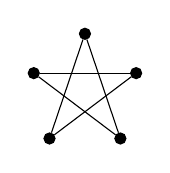
\begin{tikzpicture}[baseline=(current bounding box.center), vertex/.style={draw, fill, circle, inner sep=0pt, minimum size=4pt}]
\node (a) at (0,0.33) [vertex] {};
\node (b) at (-0.45,-1) [vertex] {};
\node (c) at (0.45,-1) [vertex] {};
\node (d) at (-0.65,-0.17) [vertex] {};
\node (e) at (0.65,-0.17) [vertex] {};

\draw (a) to (b);
\draw (a) to (c);
\draw (d) to (e);
\draw (d) to (c);
\draw (e) to (b);
\end{tikzpicture}
\hspace{1cm}
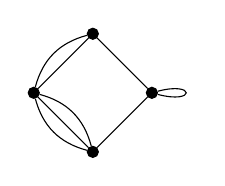
\begin{tikzpicture}[baseline=(current bounding box.center), vertex/.style={draw, fill, circle, inner sep=0pt, minimum size=4pt}]
\node (a) at (-0.75,0) [vertex] {};
\node (b) at (0.75,0) [vertex] {};
\node (c) at (0,0.75) [vertex] {};
\node (d) at (0,-0.75) [vertex] {};

\draw[bend left] (a) to (c);
\draw (a) to (c);
\draw[bend left] (a) to (d);
\draw (a) to (d);
\draw[bend right] (a) to (d);
\draw (b) to [loop right] (b);
\draw (c) to (b);
\draw (d) to (b);
\end{tikzpicture}
\hspace{1cm}

\begin{tikzpicture}[baseline=(current bounding box.center), vertex/.style={draw, fill, circle, inner sep=0pt, minimum size=4pt}]
\node (a) at (0.5,0) [vertex] {};
\node (b) at (-0.5,0) [vertex] {};
\node (c) at (0.3,1) [vertex] {};
\node (d) at (-0.3,1) [vertex] {};

\draw (a) to [bend left] (b);
\end{tikzpicture}
\end{center}
\end{example}

Note that Definition~\ref{def:graph} also supposes that the set of edges $E$ consists of \emph{unordered} pairs. By our definition, if an edge exists between vertices $u$ and $v$, then this means that another edge implicitly exists between $v$ and $u$.

If we instead require that $E$ consists of \emph{ordered} pairs, then the existence of an edge between vertices $u$ and $v$ does not necessarily imply the existence of an edge between $v$ and $u$. We say that such graphs are \emph{directed}, because the direction of each edge in the set $E$ matters when we move between vertices.

\begin{example}
Of the following graphs, the two leftmost graphs are undirected, while the two rightmost graphs are directed. In fact, the rightmost graph is the directed equivalent of the leftmost graph.

\begin{center}
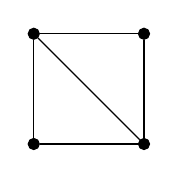
\begin{tikzpicture}[baseline=(current bounding box.center), vertex/.style={draw, fill, circle, inner sep=0pt, minimum size=4pt}]
\node (a) at (0,0) [vertex] {};
\node (b) at (1.4,0) [vertex] {};
\node (c) at (0,1.4) [vertex] {};
\node (d) at (1.4,1.4) [vertex] {};

\draw (a) to (b);
\draw (a) to (c);
\draw (b) to (d);
\draw (c) to (d);
\draw (b) to (c);
\end{tikzpicture}
\hspace{1cm}
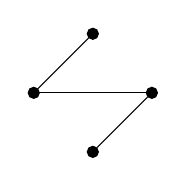
\begin{tikzpicture}[baseline=(current bounding box.center), vertex/.style={draw, fill, circle, inner sep=0pt, minimum size=4pt}]
\node (a) at (-0.75,0) [vertex] {};
\node (b) at (0.75,0) [vertex] {};
\node (c) at (0,0.75) [vertex] {};
\node (d) at (0,-0.75) [vertex] {};

\draw (a) to (b);
\draw (a) to (c);
\draw (d) to (b);
\end{tikzpicture}
\hspace{1cm}
\begin{tikzpicture}[baseline=(current bounding box.center), vertex/.style={draw, fill, circle, inner sep=0pt, minimum size=4pt}]
\node (a) at (0,0) [vertex] {};
\node (b) at (1.4,0.7) [vertex] {};
\node (c) at (0,1.4) [vertex] {};

\draw[-Latex] (a) to (b);
\draw[-Latex] (b) to (c);
\draw[-Latex] (c) to (a);
\end{tikzpicture}
\hspace{1cm}
\begin{tikzpicture}[baseline=(current bounding box.center), vertex/.style={draw, fill, circle, inner sep=0pt, minimum size=4pt}]
\node (a) at (0,0) [vertex] {};
\node (b) at (1.4,0) [vertex] {};
\node (c) at (0,1.4) [vertex] {};
\node (d) at (1.4,1.4) [vertex] {};

\draw[-Latex] (a) to (b);
\draw[-Latex] (b) to (d);
\draw[-Latex] (d) to (c);
\draw[-Latex] (c) to (a);
\draw[-Latex] (b) to [bend left] (a);
\draw[-Latex] (d) to [bend left] (b);
\draw[-Latex] (c) to [bend left] (d);
\draw[-Latex] (a) to [bend left] (c);
\draw[-Latex] (c) to [bend left] (b);
\draw[-Latex] (b) to [bend left] (c);
\end{tikzpicture}
\end{center}
\end{example}

If a graph, whether undirected or directed, has the property that we can reach any vertex from any other vertex by way of following some sequence of edges, then we say that graph is \emph{connected}. Determining whether a directed graph is connected is somewhat more difficult than in the undirected case, since we may not be able to follow the same sequence of directed edges between vertices $v$ and $u$ as we could between $u$ and $v$.

If we have two graphs $G = (V, E)$ and $H = (V', E')$ where $V' \subseteq V$ and $E' \subseteq E$, then we say that $H$ is a \emph{subgraph} of $G$. In other words, $H$ is a copy of $G$ with vertices or edges (or both) removed. Note that if we remove some vertex, then we must also remove any edges that were incident to the removed vertex.

\begin{example}
The leftmost graph contains the two rightmost graphs as subgraphs. Observe that the five edges connecting the inner subgraph to the outer subgraph were removed and do not appear in either subgraph.

\begin{center}
\begin{tikzpicture}[baseline=(current bounding box.center), vertex/.style={draw, fill, circle, inner sep=0pt, minimum size=4pt}]
\graph [nodes={fill, circle, inner sep=0pt, minimum size=4pt}, radius=0.75cm, empty nodes, clockwise] {
	subgraph C_n [n=5,name=A, radius=0.75cm]; 
	subgraph I_n [n=5,name=B, radius=0.4cm];
	\foreach \i [evaluate={\j=int(mod(\i+2,5)+1);}] in {1,...,5}{
		A \i -- B \i;
		B \i -- B \j;
	}
	};
\end{tikzpicture}
\hspace{1cm}
\begin{tikzpicture}[baseline=(current bounding box.center), vertex/.style={draw, fill, circle, inner sep=0pt, minimum size=4pt}]
\graph [nodes={fill, circle, inner sep=0pt, minimum size=4pt}, radius=0.75cm, empty nodes, clockwise] {
	subgraph I_n [n=5,name=B, radius=0.4cm];
	\foreach \i [evaluate={\j=int(mod(\i+2,5)+1);}] in {1,...,5}{
		B \i -- B \j;
	}
	};
\end{tikzpicture}
\hspace{1cm}
\begin{tikzpicture}[baseline=(current bounding box.center)]
	\graph[nodes={fill, circle, inner sep=0pt, minimum size=4pt}, radius=0.75cm, empty nodes] { subgraph C_n [n=5, clockwise] };
\end{tikzpicture}
\end{center}
\end{example}

Given a graph $G = (V, E)$, two vertices $u, v \in V$, and a number $n \in \mathbb{N}$, a \emph{path} of length $n$ from vertex $u$ to vertex $v$ is a sequence of edges $(e_{1}, \dots, e_{n})$ such that $e_{1} = \{u, w_{1}\}$, $e_{2} = \{w_{1}, w_{2}\}$, \dots, and $e_{n} = \{w_{n-1}, v\}$, where $w_{1}, \dots, w_{n-1} \in V$. We can define paths in directed graphs by making the appropriate changes to the individual edges.

We say that a path of length $n$ from a vertex $u$ to a vertex $v$ is called a \emph{circuit} (or a \emph{cycle}) if $u = v$ and $n > 0$.

If no edge in the path or circuit is included more than once, then we say that the path or circuit is \emph{simple}.

\begin{example}
In the following graph, we see that (among many others) there exist
\begin{itemize}
\item paths $a$--$b$, $a$--$c$--$e$--$g$, $c$--$e$--$c$--$a$, and $f$--$g$--$f$; 
\item simple paths $b$--$a$--$c$--$e$, $d$--$a$--$b$, and $f$--$e$--$c$; 
\item circuits $a$--$c$--$e$--$c$--$a$ and $a$--$d$--$b$--$a$--$c$--$a$; and
\item simple circuits $a$--$b$--$d$--$a$ and $e$--$f$--$g$--$e$.
\end{itemize}
\begin{center}
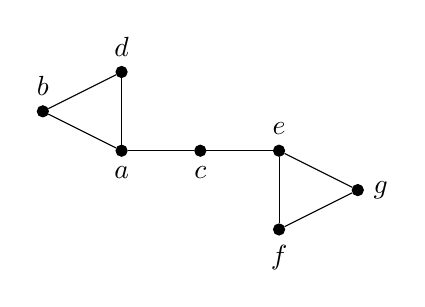
\begin{tikzpicture}[baseline=(current bounding box.center), vertex/.style={draw, fill, circle, inner sep=0pt, minimum size=4pt}]
\node (a) at (0,0) [vertex,label=below:$a$] {};
\node (b) at (-1,0.5) [vertex,label=above:$b$] {};
\node (c) at (1,0) [vertex,label=below:$c$] {};
\node (d) at (0,1) [vertex,label=above:$d$] {};
\node (e) at (2,0) [vertex,label=above:$e$] {};
\node (f) at (2,-1) [vertex,label=below:$f$] {};
\node (g) at (3,-0.5) [vertex,label=right:$g$] {};

\draw (a) to (b);
\draw (a) to (c);
\draw (a) to (d);
\draw (b) to (d);
\draw (e) to (c);
\draw (e) to (f);
\draw (e) to (g);
\draw (f) to (g);
\end{tikzpicture}
\end{center}
\end{example}